%\documentclass[12pt,a4paper]{report}
%\usepackage[utf8]{inputenc}
%\usepackage[english]{babel}
%\usepackage{amsmath}
%\usepackage{amsfonts}
%\usepackage{amssymb}
%\usepackage{graphicx}
%\usepackage{eurosym}
%\usepackage[left=2cm,right=2cm,top=2cm,bottom=2cm]{geometry}
%\usepackage{wrapfig}
%\usepackage{mathdots}
%\usepackage{caption}
%\usepackage{cite}
%\usepackage{mathrsfs}
%\usepackage{float}
%\author{Eva María Urbano González}
%\title{Data Link Layer Protocol}
%\begin{document}
%\maketitle
%\tableofcontents
%\listoffigures
%\listoftables
%\chapter{DLL}
\subsection{Functions of the DLL}
The explained functions are:
\begin{itemize}
\item \textbf{Framing}: Data-link layer takes packets from Network Layer and encapsulates them into Frames.Then, it sends each frame bit-by-bit on the hardware. At receiver end, data link layer picks up signals from hardware and assembles them into frames.
\item \textbf{Adressing}: Each device on a network has a unique number, usually called a hardware address or MAC address, that is used by the data link layer protocol to ensure that data intended for a specific machine gets to it properly.
\item \textbf{Synchronization}: When data frames are sent on the link, both machines must be synchronized in order to transfer to take place.
\item \textbf{Error control}: Sometimes signals may have encountered problem in transition and the bits are flipped. These errors are detected and attempted to recover actual data bits.
\item \textbf{Flow control}: Stations on same link may have different speed or capacity. Data-link layer ensures flow control that enables both machine to exchange data on same speed. 
 \end{itemize}
\subsection{Working procedure}
Working procedure is explained deeply now. All the images have been extracted from\cite{Forouzan2012}.
\subsubsection{Simplest Protocol}
This protocol has no error or flow control. It is supposed that the frames are traveling only in one direction, from the sender to the receiver. It is also supposed that the receiver can immediately handle the frames received, so there is no overwhelming. The DLL of the sender site gets data from its network layer, makes a frame out of the data and sends it.
The DLL at the receiver site receives a frame from its physical layer, extracts data from the frame and delivers the data to its network layer. The problem here is that the sender site cannot send a frame until its network layer has a data packet to send and the receiver site cannot deliver a data packet to its network layer until a frame arrives. There is the need to introduce the idea of events in the protocol. The
procedure at the sender site is constantly running; there is no action until there is a request
from the network layer. The procedure at the receiver site is also constantly running, but
there is no action until notification from the physical layer arrives.
\begin{figure}[H]
\begin{center}
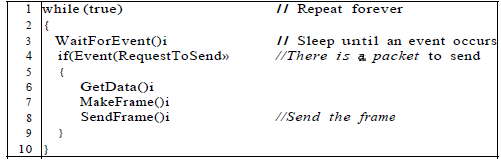
\includegraphics[scale=1]{simplestsender.PNG}
\caption{Sender algorithm for the simplest protocol.}
\end{center}
\end{figure}
\begin{figure}[H]
\begin{center}
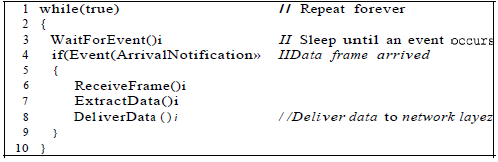
\includegraphics[scale=1]{simplestreceiver.PNG}
\caption{Receiver algorithm for the simplest protocol.}
\end{center}
\end{figure}
\subsubsection{Stop-and-Wait Protocol}
If data frames arrive at the receiver site faster than they can be processed, the frames
must be stored until their use. Normally, the receiver does not have enough storage
space, especially if it is receiving data from many sources. This may result in either the
discarding of frames or denial of service. To prevent the receiver from becoming overwhelmed
with frames,we somehow need to tell the sender to slow down. There must be
feedback from the receiver to the sender.\\
In the Stop-and-Wait Protocol the sends one frame, stops until it receives confirmation from the receiver and then sends the next frame. We still have unidirectional communication
for data frames, but auxiliary ACK frames (simple tokens of acknowledgment) travel
from the other direction. We add flow control to our previous protocol. In this case the algorithms of the sender and the receiver are the following ones. 
\begin{figure}[H]
\begin{center}
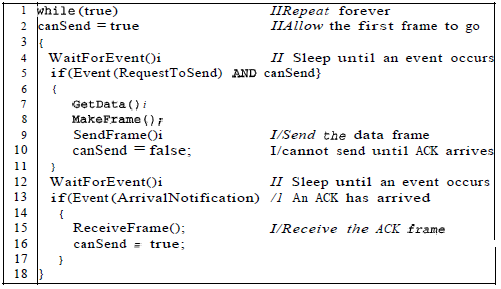
\includegraphics[scale=1]{sendersawp.PNG} 
\caption{Sender algorithm for the Stop-and-Wait Protocol.}
\end{center}
\end{figure} 
\begin{figure}[H]
\begin{center}
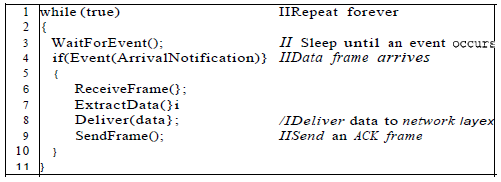
\includegraphics[scale=1]{receiversawp.PNG} 
\caption{Receiver algorithm for the Stop-and-Wait Protocol.}
\end{center}
\end{figure}
The two protocols explained are protocols that can be suitable for noiseless channels. However, noiseless channels are nonexistent. There is a need to add error control to the protocol. Three protocols are discussed with the aim of doing so.
\subsubsection{Stop-and-Wait Automatic Repeat Request}
The Stop-and Wait ARQ adds a simple error control mechanism to the Stop-and-Wait Protocol. To detect and correct corrupted frames, we need to add redundancy bits to our data
frame. When the frame arrives at the receiver site, it is checked and if
it is corrupted, it is silently discarded. The detection of errors in this protocol is manifested
by the silence of the receiver. Frames are also numbered so if the
receiver receives a data frame that is out of order, this means that frames were either
lost or duplicated. What is done to solve the error is that when the sender sends a frame, it    keeps a copy of the sent frame. At the same time, it starts
a timer. If the timer expires and there is no ACK for the sent frame, the frame is resent, the
copy is held, and the timer is restarted. Since the protocol uses the stop-and-wait mechanism,
there is only one specific frame that needs an ACK even though several copies of
the same frame can be in the network. Since an ACK frame can also be corrupted and lost, it too needs redundancy bits
and a sequence number. In the following figure is possible to see more clearly what is going on with this protocol. 
\begin{figure}[H]
\begin{center}
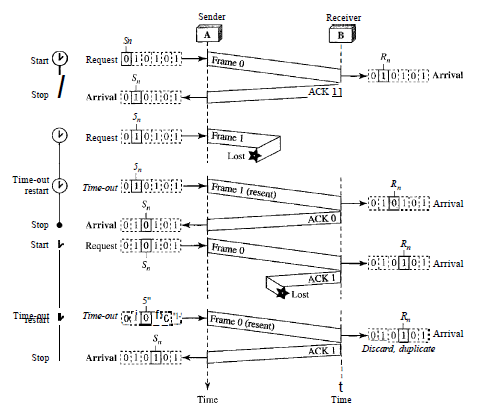
\includegraphics[scale=1]{flowdiagram.PNG} 
\caption{Flow diagram of the Stop-and Wait ARQ.}
\end{center}
\end{figure}
The main problem of this protocol is its efficiency. The Stop-and-Wait ARQ is very inneficinet if our channel is thick and long. The product of thickness and longitud is called the bandwidth-delay product. We can think of the channel as a pipe. The
bandwidth-delay product then is the volume of the pipe in bits. The pipe is always there.
If we do not use it, we are inefficient. 
\subsubsection{Go-Back-N Automatic Repeat Request}
To improve the efficiency of transmission (filling the pipe), multiple frames must be in
transition while waiting for acknowledgment. In other words, we need to let more than
one frame be outstanding to keep the channel busy while the sender is waiting for
acknowledgment. In the Go-Back-N Automatic Repeat Request the sender sends several frames before receiving acknowledgments. It also keeps a copy of these frames until the acknowledgments
arrive. Although there can be a timer for each frame that is sent, in this protocol only one is used. The reason is that the timer for the first outstanding frame always expires first and then all outstanding frames when this timer expires are sent again. The receiver sends a positive acknowledgment if a frame has arrived safe and sound
and in order. If a frame is damaged or is received out of order, the receiver is silent and
will discard all subsequent frames until it receives the one it is expecting. The silence of
the receiver causes the timer of the unacknowledged frame at the sender site to expire.
This, in turn, causes the sender to go back and resend all frames, beginning with the one
with the expired timer. The receiver does not have to acknowledge each frame received.
It can send one cumulative acknowledgment for several frames. That is the reason why the protocol is called Go-Back-N. The flow diagram and the and algorithms of the sender and the receiver are shown next. 
\begin{figure}[H]
\begin{center}
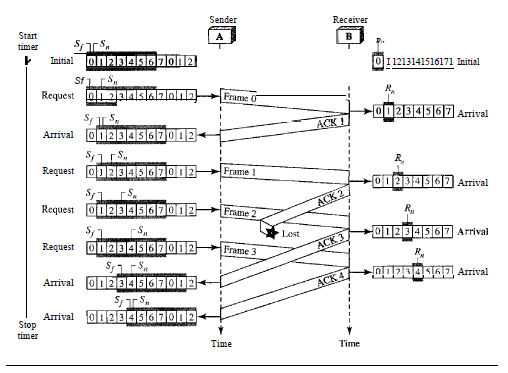
\includegraphics[scale=1]{diagramN.PNG}  
\caption{Flow diagram of the Go-Back-N ARQ.}
\end{center}
\end{figure} 
\begin{figure}[H]
\begin{center}
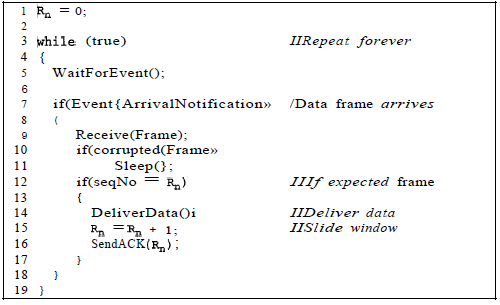
\includegraphics[scale=1]{receiverN.PNG} 
\caption{Receiver algorithm for the Go-Back-N ARQ.}
\end{center}
\end{figure} 
\begin{figure}[H]
\begin{center}
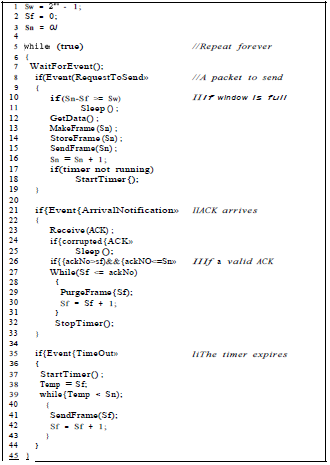
\includegraphics[scale=1]{SenderN.PNG} 
\caption{Sender algorithm for the Go-Back-N ARQ.}
\end{center}
\end{figure}
\subsubsection{Selective Repeat Automatic Repeat Request}
Go-Back-N ARQ simplifies the process at the receiver site. The receiver keeps track of
only one variable, and there is no need to buffer out-of-order frames; they are simply
discarded. However, this protocol is very inefficient for a noisy link. In a noisy link a
frame has a higher probability of damage, which means the resending of multiple frames. In the case of these protocol, the Selective Repeat ARQ, the processing at the receiver is more complex but is more efficient for noisy links. The Selective Repeat Protocol allows a number of frames to arrive out of order and be kept until there is a set of in-order frames to be
delivered to the network layer. The handling of the request event is similar to that of the previous protocol except
that one timer is started for each frame sent. The arrival event is more complicated here. An ACK
or a NAK frame may arrive. If a valid NAK frame arrives, the corresponding frame is resent. If a valid ACK arrives the corresponding timer stops. When the time for a frame has expire, only this frame is resent.
\begin{figure}[H]
\begin{center}
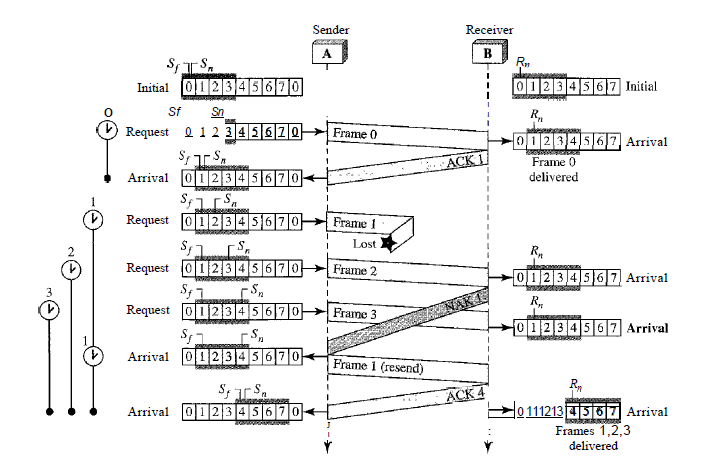
\includegraphics[scale=0.8]{flowselective.PNG}  
\caption{Flow diagram of the Selective Repeat ARQ.}
\end{center}
\end{figure}
\begin{figure}[H]
\begin{center}
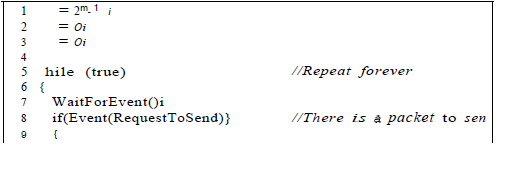
\includegraphics[scale=0.8]{senderselective1.PNG}
\end{center} 
\end{figure}
\begin{figure}[H]
\begin{center}
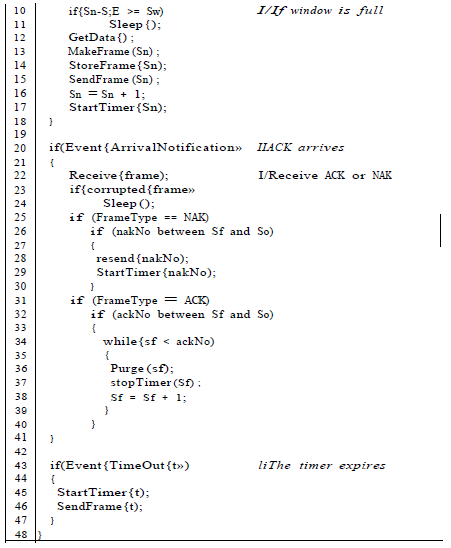
\includegraphics[scale=1]{senderselective2.PNG} 
\caption{Sender algorithm for the Selective Repeat ARQ.}
\end{center}
\end{figure}
\begin{figure}[H]
\begin{center}
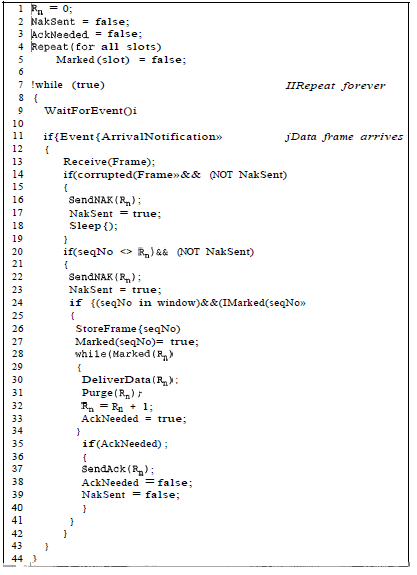
\includegraphics[scale=1]{receiverselective.PNG}  
\caption{Receiver algorithm for the Selective Repeat ARQ.}
\end{center}
\end{figure}
\subsubsection{Bidirecional links: Piggybacking}
Piggybacking is not a protocol, is a technique. All que protocols explained until now are all unidirectional: data frames flow
in only one direction although control information such as ACK and NAK frames can
travel in the other direction. In real life, data frames are normally flowing in both directions:
from node A to node B and from node B to node A. This means that the control
information also needs to flow in both directions. Piggybacking is usedto improve the efficiency of the bidirectional protocols. When a frame is carrying
data from A to B, it can also carry control information about arrived (or lost) frames
from B; when a frame is carrying data from B to A, it can also carry control information
about the arrived (or lost) frames from A.
\subsubsection{Working procedure ranking}
Now its time to choose the working procedure that best fits the needs of the mission. To do so, an OWA (Ordered Weighted Average) will be used. The criteria to consider is the following one:
\begin{itemize}
\item Efficiency: This fact deals with how the channel is being used. Protocols will be classified as non-efficient or efficient. 
\item Time: This fact deals about the time needed to transmit the data satisfactory.
\item Error correction: Deals about whether a protocol can correct an error of transmission or not.
\end{itemize}
It is important also to take into account that the protocol to use should have a flow control, that is, should know if the receiver is available or not to receive the data. For this reason the Simplest Protocol is rejected and won't be studied in the OWA. Regarding the factors of the OWA, all of them will be rated from 0 to 1. In this project the fact of transmitting the data without errors is more important than transmitting it fast, as is possible to appreciate un the project charter ( the latency can be relative high, but incorrect information is useless). The efficiency of the protocol is very important too, because the less the efficiency the less power provided by the CubeSat is being used. Since the CubeSat has limited space, ideally al the power it can gives for transmittion will be used for it. Then, the weights of the different factors are the following ones:
\begin{itemize}
\item Efficiency: 40
\item Time: 30
\item Error correction: 60
\end{itemize} 
In the following table the rating of each protocol together with the corresponding OWA is shown. 
\begin{table}[H]
\begin{center}
\begin{tabular}{ | c | c | c | c | c |}
\hline
Protocol&Efficiency&Time&Error correction&OWA\\
\hline
Stop-and-Wait Protocol&0&0&0&0\\
\hline
Stop-and-Wait ARQ&0&0&1&0,46\\
\hline
Go-Back-N ARQ&1&0&1&0.69\\
\hline
Selective Repeat ARQ&1&1&1&1\\
\hline
\end{tabular}
\caption{OWA of the DLL protocols.}
\end{center}
\end{table} 
Then, the ranking of working procedures is the following one: 
\begin{table}[H]
\begin{center}
\begin{tabular}{|c|c|}
\hline
\textbf{1}&Selective Repeat ARQ\\
\hline
\textbf{2}&Go-Back-N ARQ\\
\hline
\textbf{3}&Stop-and-Wait ARQ\\
\hline
\textbf{4}&Stop-and-Wait Protocol\\
\hline
\end{tabular}
\caption{Ranking of working procedures}
\end{center}
\end{table}
It has to be said that when dealing with bidirecional links piggybacking technique will be used if possible.
\subsection{Protocols}
The standards of the CCSDS will be followed in order to allow interoperability with other satellites such as the one of the client. The CCSDS has developed four protocols for the Data Link Protocol Sublayer of the Data Link Layer\cite{Secretariat2014}:
\begin{itemize}
\item TM Space Data Link Protocol
\item TC Space Data Link Protocol
\item AOS Space Data Link Protocol
\item Proximity-1 Space Link Protocol-Data Link Layer
\end{itemize}
These protocols provide the capability to send data over a single space link. TM, TC, and AOS can have secured user data into a frame using the Space Data Link Security (SDLS) Protocol.\\
 CCSDS has also developed three standards for the Synchronization and Channel Coding Sublayer of the DLL:
 \begin{itemize}
 \item TM Synchronization and Channel Coding
 \item TC Synchronization and Channel Coding
 \item Proximity-1 Space Link Protocol—Coding and Synchronization Layer
 \end{itemize}
TM Synchronization and Channel Coding is used with the TM or AOS Space Data Link
Protocol, TC Synchronization and Channel Coding is used with the TC Space Data Link Protocol and the Proximity-1 Space Link Protocol—Coding and Synchronization Layer is
used with the Proximity-1 Space Link Protocol—Data Link Layer. This can be seen better in the following image.\\
\begin{figure}[H]
\begin{center}
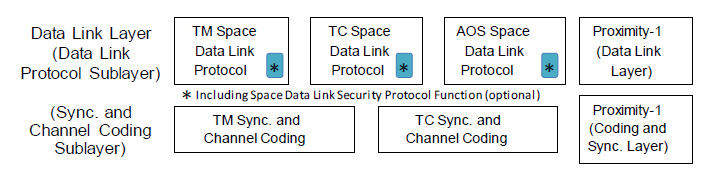
\includegraphics[scale=0.9]{DLLCCSDS.PNG}   
\caption{DLL of the CCSDS.}
\end{center}
\end{figure}
Now the reliability of each of the protocols of the Data Link Protocol Sublayer will be compared in order to know which one is the best of them. This will be done because reliability is the most important feature of the DLL.
\begin{table}[H]
\begin{center}
\begin{tabular}{|c|c|}
\hline
\textbf{Protocol}&\textbf{System used for reliability}\\
\hline
TM&Stop-and-Wait Protocol\\
\hline
TC&Type-A: Go-Back-N ARQ, Type-B:Stop-and-Wait Protocol\\
\hline
AOS&Stop-and-Wait Protocol\\
\hline
Proximity-1&Go-Back-N ARQ\\
\hline
\end{tabular}
\caption{Reliability of CCSDS protocols}
\end{center}
\end{table}
According to the table and to the ranking of working procedures done previously, only TC Type-A and Proximity-1 will be considered from now on. Security is another important feature to take into account when taking this decision. TM Space Data Link Protocol has provision for inserting secured data into a frame using the Space Data Link Security (SDLS) Protocol. However, there have been no security requirements to date established for Proximity-1. The SLDS protocol can provide security services, such as authentication and confidentiality for TC Transfer Frames (it can also do it with TM and AOS, that have been previously discharted). Both the TC and the Proximity-1 use variable-lenght Transfer Frames to facilitate reception of short messages with short delay. Another key feature to take into account when deciding a protocol, is the concept of "Virtual Channels". The
Virtual Channel facility allows one Physical Channel (a stream of bits transferred over a
space link in a single direction) to be shared among multiple higher-layer data streams, each
of which may have different service requirements. A single Physical Channel may therefore
be divided into several separate logical data channels, each known as a Virtual Channel
(VC). The TC has the following identifiers: the Transfer Frame Version Number (TFVN), the Spacecraft Identifier (SCID), and the Virtual Channel Identifier (VCID). It also uses an optional identifier, called the Multiplexer Access Point Identifier (MAP ID), that is used to create multiple streams of data within a Virtual Channel. In contrast, the Proximity-1 uses a triad of multiplexing capabilities, which is incorporated for specific funcionality within the link. The Spacecraft Identifier (SCID) identifies the source or destination of Transfer Frames transported in the link connection based upon the Source-or-Destination Identifier. The Pysical Channel Identifier (PCID) provides up to two independently multiplexed channels. The Port ID provides the means to route user data internally to specific logic ports, such as applications or transport processes, or to physical ports, such as onboard buses or physical connections. Now a table with the identifiers of the TC and the Proximity-1 will be shown:
\begin{table}[H]
\begin{center}
\begin{tabular}{|c|c|c|}
\hline
Identifiers&TC Space Data Link Protocol&Proximity-1 Space Link Protocol- Data Link Layer\\
\hline
TFVN&00&10\\
\hline
SCID&0 to 1023&0 to 2013\\
\hline
PCID&N/A&0 to 1\\
\hline
VCID&0 to 63&N/A\\
\hline
MAP ID&0 to 63&N/A\\
\hline
Port identifier&N/A&0 to 7\\
\hline
\end{tabular}
\caption{Identifiers of TC and Proximity-1 Space Data Link Layer Protocols}
\end{center}
\end{table} 
Having Virtual Channels is important for the mission that is exposed in this project because it allows having more than one stream of bits to take place at the same time, that is to say that more than one client can communicate with their satellite without having to wait for another client to finish.\\
The decision taken is to use the TC Space Data Link Protocol with the TC sync. and channel coding together with the Space Data Link Security Protocol. The reasons for doing so are mainly:
\begin{itemize}
\item Security: Incorporing the SLDS authentication and confidentality is provided.
\item More virtual channels: This feature allow more clients communicating with their satellites at the same time.
\end{itemize}

\subsection{TC Space Data Link Protocol}
Now some specifications of the chosen protocol will be exposed in order to know how it is structured and how many bits it adds to the original data. Further information of the protocol can be found in \cite{CCSDS2010}. The protocol specifications will be explained when it is used with the support of the SDLS protocol. In this section is important to know that 1 octet is an eight-bit word. The structure of the transfer frame in this protocol is the following one: 
\begin{figure}[H]
\begin{center}
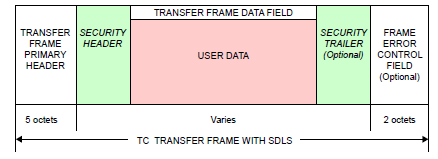
\includegraphics[scale=1]{transferfram.PNG}    
\caption{Transfer frame structure of the TC Space DL Protocol with SDLS.}
\end{center}
\end{figure}  
In the transfer frame primary header, the following information is contained:
\begin{figure}[H]
\begin{center}
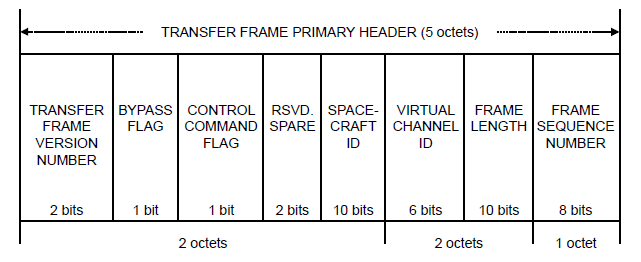
\includegraphics[scale=1]{transferframeprimaryheader.PNG}   
\caption{Transfer frame primary header.}
\end{center}
\end{figure} 
With this data, is possible to say that the TC Space Data Link Protocol will add to data coming from the Network layer at least 5 octets (40 bits).
\subsection{TC Sync and Channel Coding}
This protocol is the corresponding to the Synchronization and Channel Coding Sublayer that has be used with the TC Space and Data Link Protocol. It has functions as for example, encapsuate the data units so that the start and end can be detected by the receiving end, ensure there are sufficient bit transitions in the transmitted bit stream so that the receiver can mantain bit synchronization during the reception of the data unit, etc. In a nutshell, one instance of the Synchronization and Channel Coding Sublayer processes the data stream for a single Physical Channel, making it a stream of bits that can be transferred over a space link in a single direction. The procedures can be differenciated between the ones that occur in the sending end and the one that occur in the receiving end. The procedures are the following ones: 
\begin{figure}[H]
\begin{center}
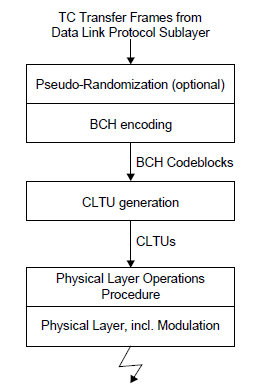
\includegraphics[scale=1]{Proceduressendingend.PNG}    
\caption{Procedure at the sending end.}
\end{center}
\end{figure}
\begin{figure}[H]
\begin{center}
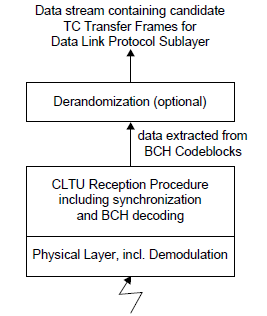
\includegraphics[scale=1]{proceduresreceivingend.PNG}  
\caption{Procedure at the receiving end.}
\end{center}
\end{figure}
Is possible to see that two packets of data are created, BCH Codeblocks and CLTUs. From the point of view of the Synchronization and Channel Coding Sublayer, the content of
the Frames parameter is a single block of data. For a single Channel Access request, the Synchronization and Channel Coding Sublayer
generates a set of BCH Codeblocks, and that set of BCH Codeblocks is placed in a single
CLTU. One of the managed parameters for the Physical Channel is the maximum length of a
CLTU. The lenght of the CLTU can be calculated as follows (in octets): 
\begin{equation}
Lenght of the CLTU=10+8\cdot(\frac{Total lenght of the frames+6}{7})
\end{equation} 
Since with the TC Space Data Link protocol the frames can have different sizes, the CLTU can also have different sizes. More information about this sublayer of the DLL can be found in reference \cite{Synchronization2012}

%\bibliographystyle{unsrt}
%\bibliography{forouzan,Secretariat2014,TC,tmsynch} 
%\end{document}